\documentclass{article}
\usepackage{graphicx}
\usepackage{xspace}
\usepackage{balance}  
\usepackage{amsmath}  
\usepackage{comment}
\usepackage{algorithm}
\usepackage[noend]{algpseudocode}
\usepackage{tablefootnote}
\usepackage{booktabs}
\usepackage{float}
\usepackage{url}
\usepackage{array}
\usepackage{cleveref}
\usepackage{pbox}
\usepackage{mdwlist}
\usepackage{cite}
\usepackage{footnote}

\begin{document}
	
\title{Interactive Machine Learning Interface}
\author{Lilong Jiang(jiang.573)}
\date{}
\maketitle
\section{Abstract}
\section{Introduction \& Motivation}
% visual data analysis is popular, business intelligence (tableau)
% motivation: interactive visualization, usability, verfication


\section{Related Work}
\cite{crotty2015vizdom} shows an interactive interface for machine learning. 
We use a classification Pima Indians Diabetes Data Set from UCI~\cite{smith1988using}.

\section{Work}
The overall space is divided into two parts: the left part shows what kind of machine learning method to run and parameters associated with the algorithm. Also users can choose different dataset and it will show the attributes of current manipulated dataset.  In general, we implement three machine learning algorithms in the frontend using javascript: K-means (Figure~\ref{fig:kmeans}), linear regression (Figure~\ref{fig:regression}) and support vector machine (SVM) (Figure~\ref{fig:svm}).  Table~\ref{table:operations} summarizes operations that users can perform with our interface. 
\begin{table}
	\begin{tabular}{l l}
		algorithms & operations  \\ \hline \hline
		k-means & \pbox{50cm}{(1) Select initial centers or generate centers randomly \\ (2) Adjust number of clusters on-line \\ (3) Colors shows different clusters} \\ \hline \hline
		linear regression & \pbox{20cm}{(1) Adjust function's intercept by moving the line \\ (2) Adjust function's slope and intercept by dragging end points \\ (3) Dynamically show the function and square loss} \\ \hline \hline
		svm & \pbox{20cm}{(1) Select kernel \\ (2) Select which features to use by dragging into or out space \\ (3) Dynamically show accuracy, precision, recall and confustion matrix}
	\end{tabular}
	\label{table:operations}
	\caption{Operations}
\end{table}

\begin{figure}[h]
	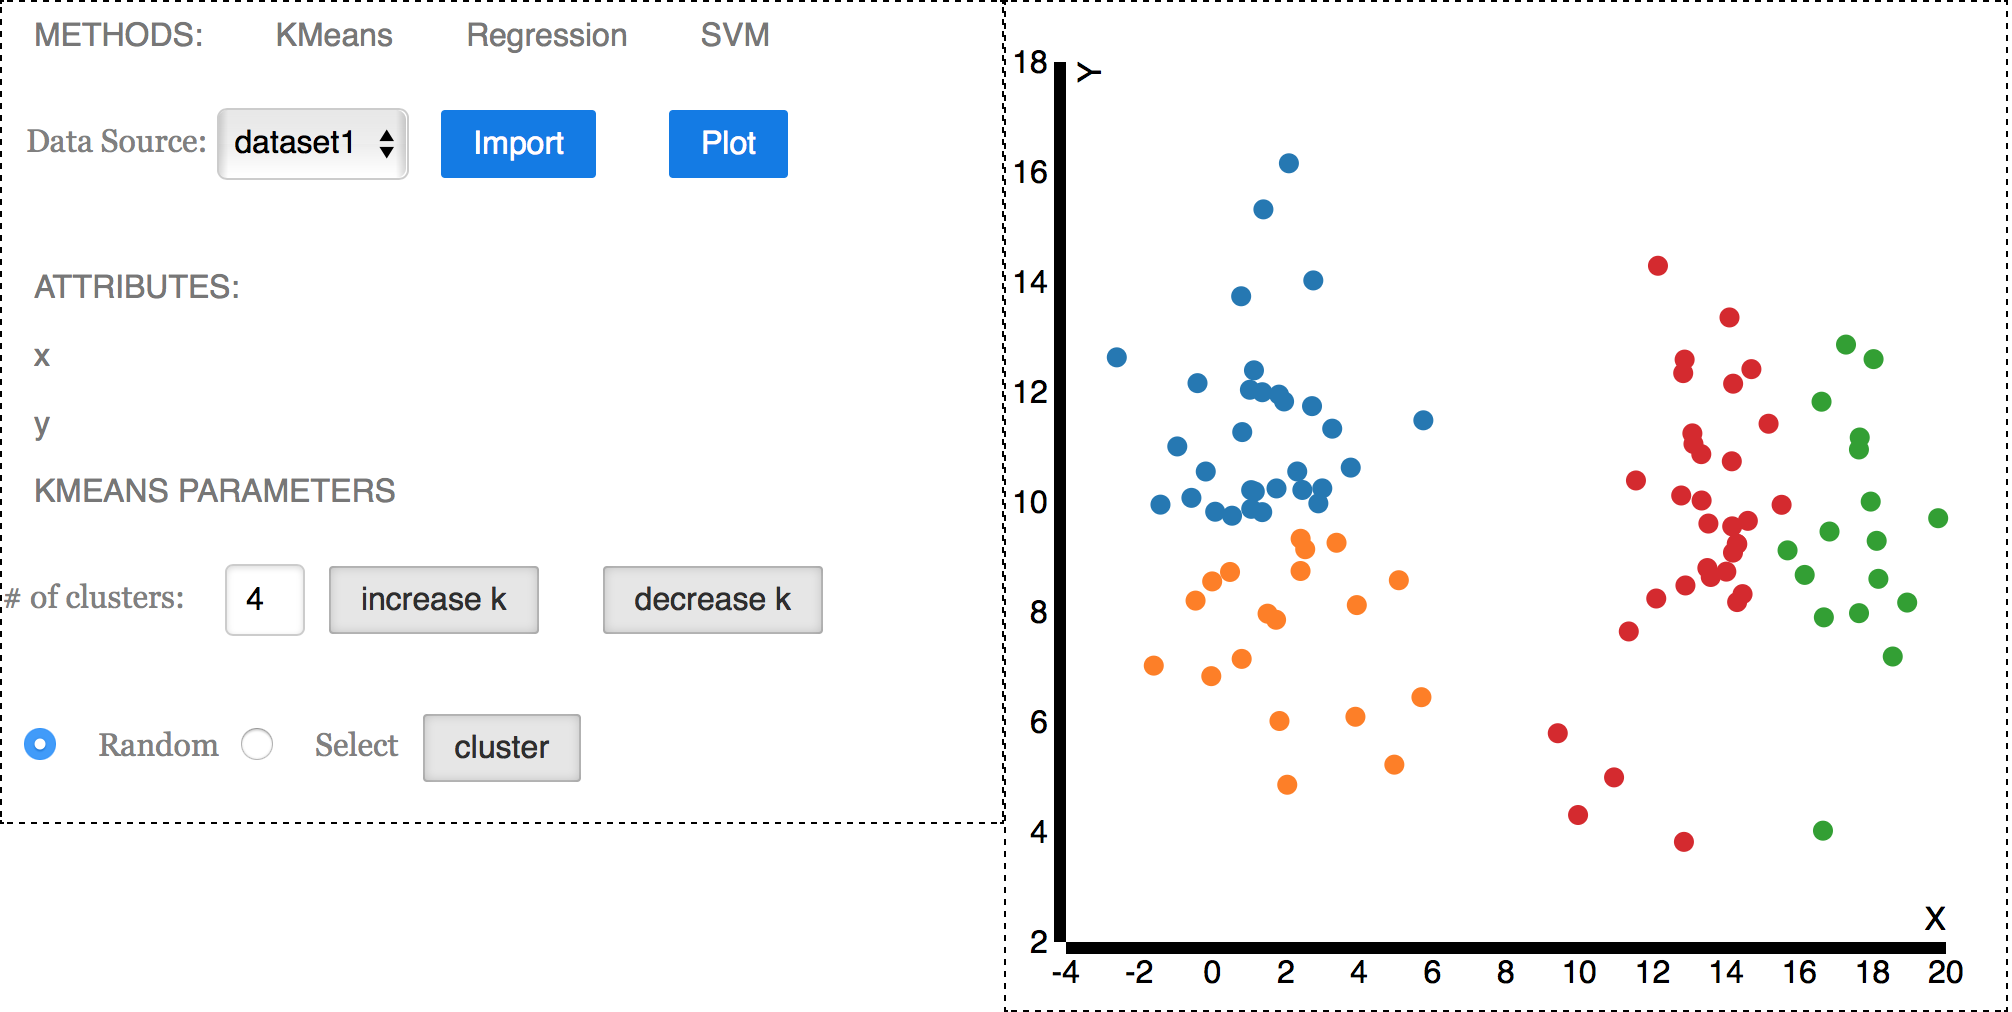
\includegraphics[width=\textwidth]{figs/kmeans}
	\label{fig:kmeans}
	\caption{K-means}
\end{figure} 
\begin{figure}[h]
	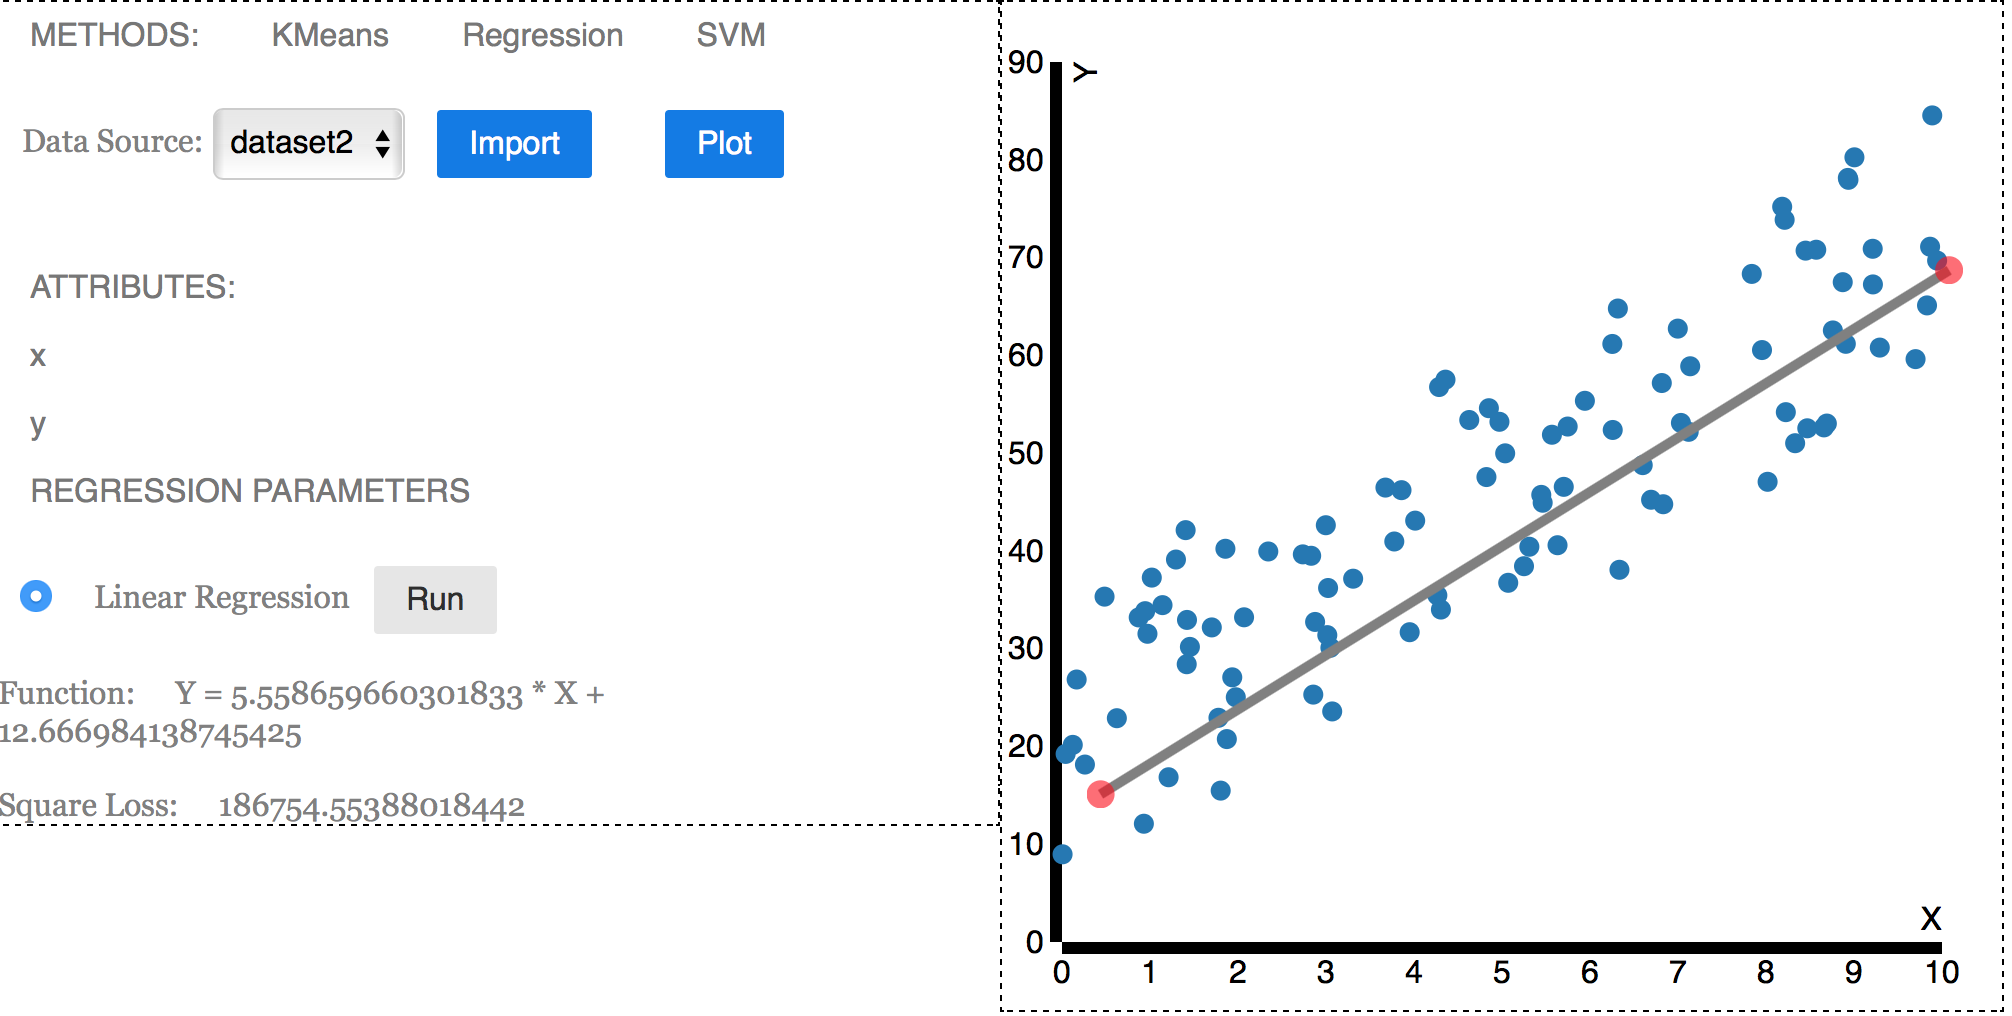
\includegraphics[width=\textwidth]{figs/linearregression}
	\label{fig:regression}
	\caption{Linear Regression}
\end{figure} 
\begin{figure}[h]
	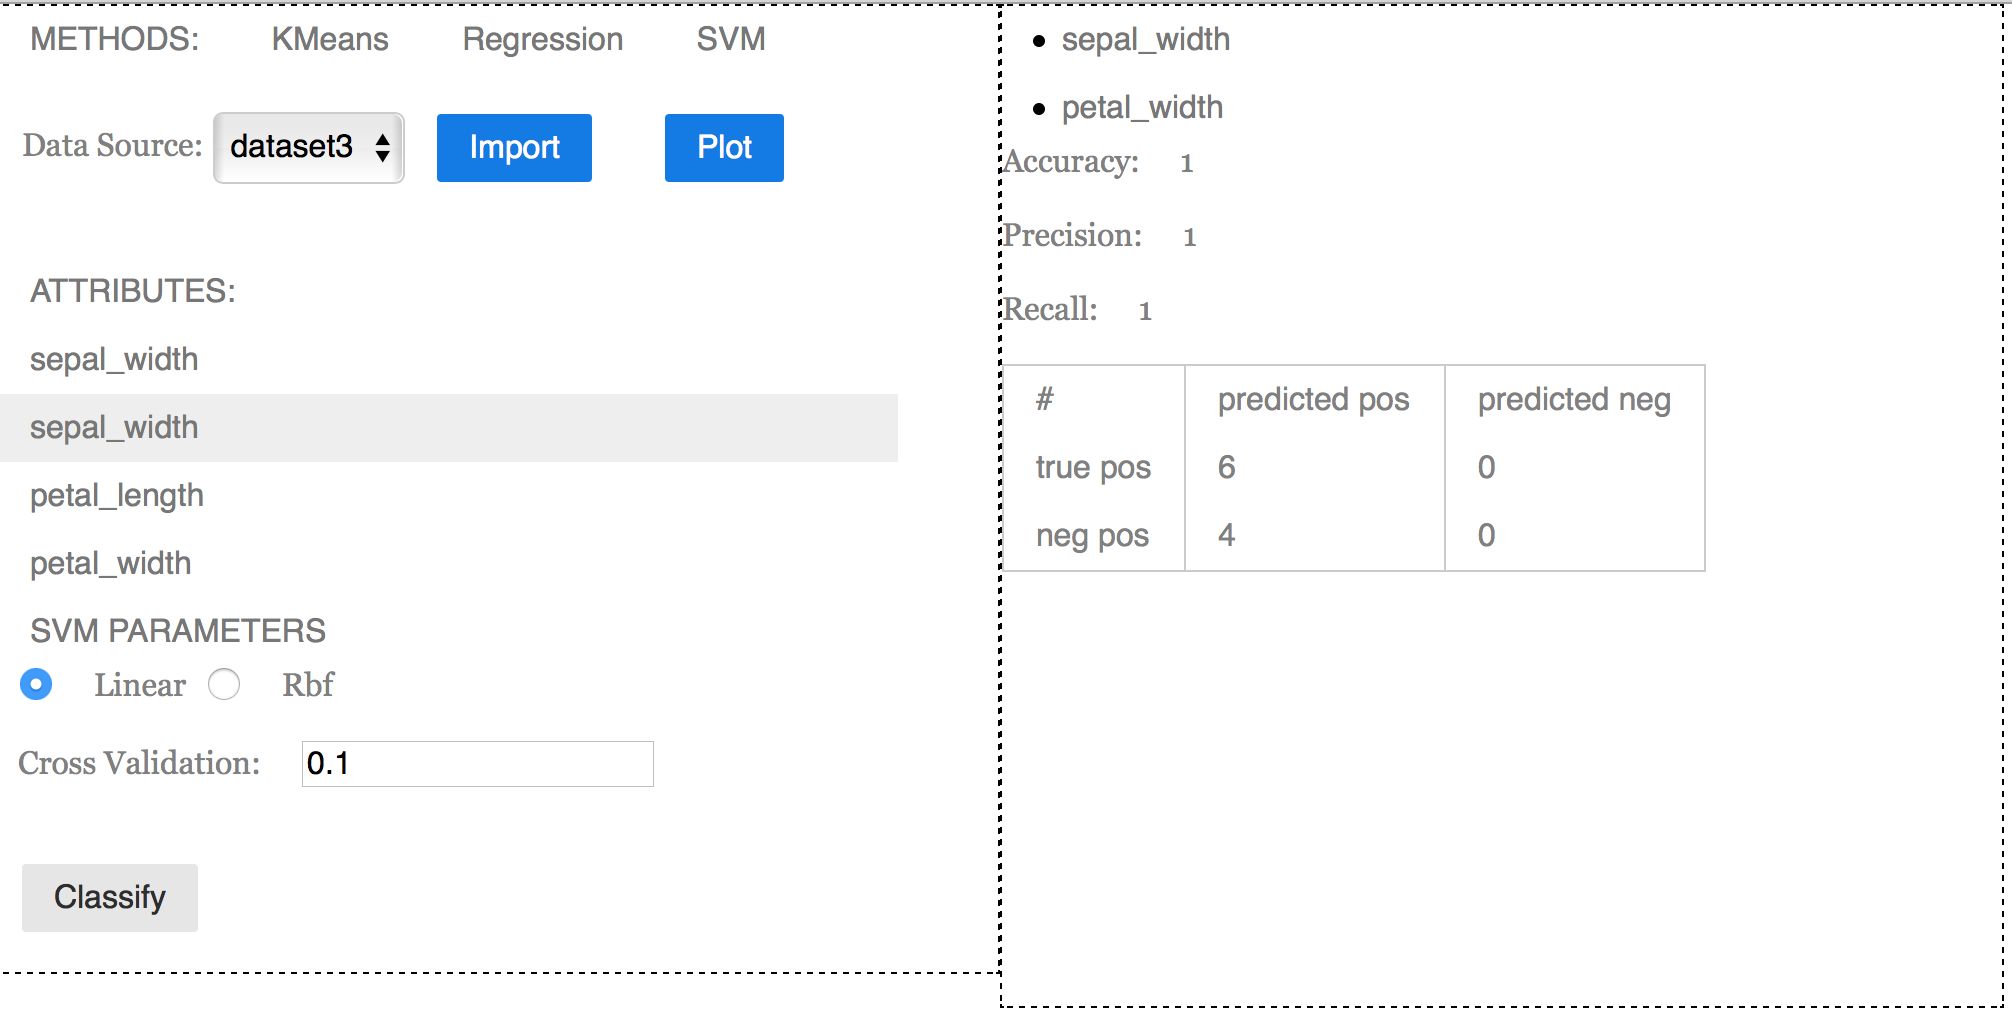
\includegraphics[width=\textwidth]{figs/svm}
	\label{fig:svm}
	\caption{SVM}
\end{figure} 

\section{Performance Experiments}
In this section, we focus on performance experiments since in the interactive environment, it is necessary to keep an interactive performance. \\
\textbf{Computer Configuration:} \\
\textbf{Dataset:} For SVM, we use Skin Segmentation Data Set from UCI~\cite{skinsegment}.  There are totally 3 numerical attributes and 2 classes. We randomly sample from both classes. \\
\textbf{Results:} \\
\begin{figure}[h]
	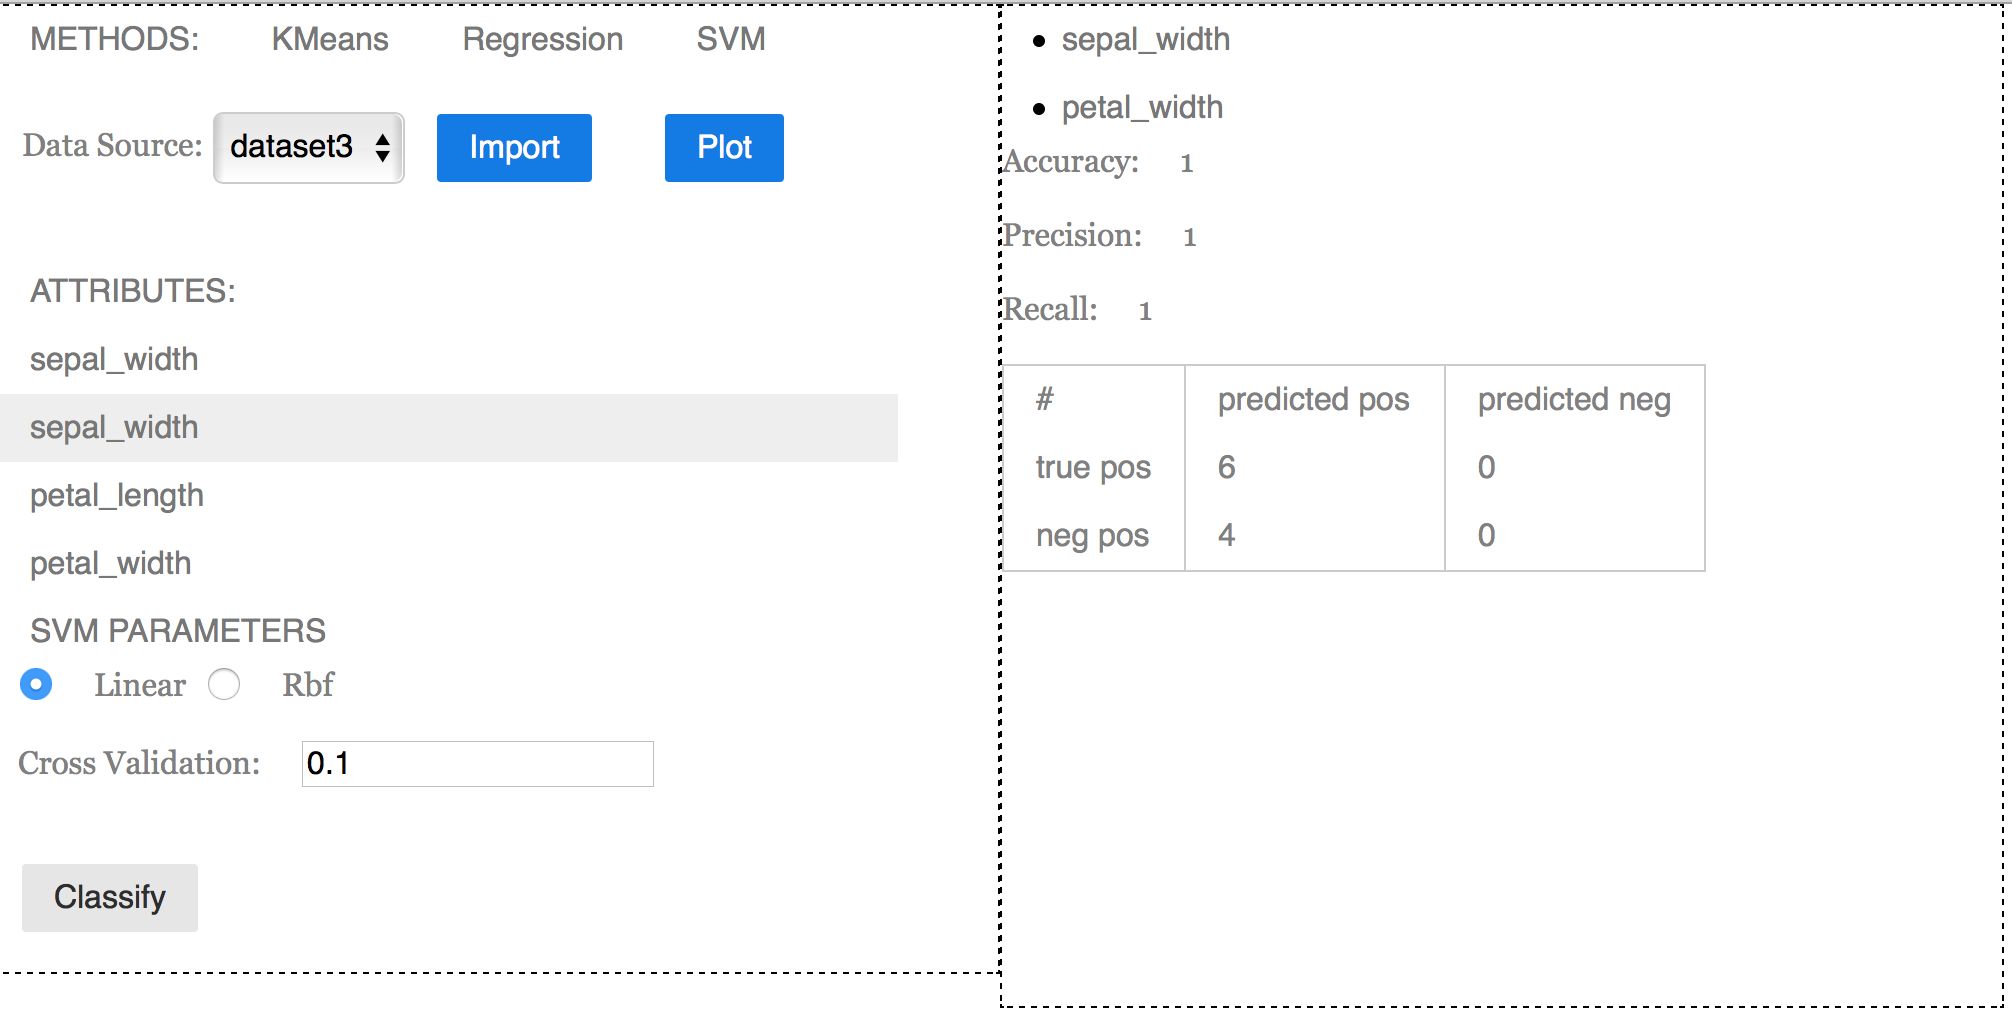
\includegraphics[width=\textwidth]{figs/svm}
	\label{fig:svm}
	\caption{SVM}
\end{figure} 

\section{Limitations \& Conclusions}
In this project, we focus on usability point. There are several limitations for this project. The first is interactive performance. The second is project issue for high-dimensional dataset. \emph{Projection} is a technique that maps high-dimensional dataset into a small set of dimensions. Some works use dimension reduction, that create latent dimensions that summarize dataset. For example, Principal Component Analysis (PCA)~\cite{jolliffe2002principal}, Multidimensional Scaling (MDS)~\cite{mead1992review}. This method can reveal hidden variables. However, the generated dimensions are usually less intuitive to users. Another method is called feature selection, which selects subset of features to explore. Interactive feature selection is often used to identify relationship between features~\cite{guo2003coordinating, yang2004value} and aid user remove redundant features and choose appropriate features. Recently, there is a work trying to allow users to craft their own projection function~\cite{gleicher2013explainers}.  All these methods can be easily incorporated into our project.  \\

\bibliography{main}
\bibliographystyle{plain}
\end{document}